\documentclass[11pt]{article}
\usepackage[utf8]{inputenc}
\usepackage{fancyhdr}
\usepackage[english]{babel}
\usepackage{graphicx}
\usepackage{array}
\usepackage{amsmath}
\usepackage{amssymb}
\usepackage{mathtools}
\usepackage{algorithmicx}
\usepackage{algpseudocode}
\renewcommand{\baselinestretch}{1.0}
\usepackage[letterpaper, margin=0.75in]{geometry}
\DeclarePairedDelimiter{\ceil}{\lceil}{\rceil}
\pagestyle{fancy}
\lhead{}
\rhead{Yu Mi, yxm319. Algorithm HW3}
\begin{document}
	\title{Homework3 for EECS 340}
	\author{Yu Mi,yxm319}
	\maketitle
\section{Sorting Leftover Elements}
\noindent \emph{Question}: Suppose that you are given an array consisting of $n$ sorted elements followed by $f(n)$ elements in an arbitrary order, where $f(n)\in O(n^{1-\epsilon})$ for some $\epsilon \in(0,1)$. Describe a method to sort the array in $O(n)$ time.

\noindent \emph{Answer}: This question describes a scenario similar to the intermediate steps of a merge sort, so that we need to solve this problem similar to the approach of a merge sort. First, we need to sort the leftover elements with merge sort, which takes $O(n^{1-\epsilon}\cdot \log n^{1-\epsilon})$ time. After that, we will need to merge the two sequence (original sorted one and the left over part) into a whole sorted sequence, which takes $O(n)$ time. To show that $O(n^{1-\epsilon}\cdot \log n^{1-\epsilon})$ takes less time than $O(n)$, we assign $g(n)=n^{1-\epsilon}\cdot \log n^{1-\epsilon}$, $h(n) = n$. Thus we have:
\begin{equation*}
	\lim_{n\to\infty} \frac{g(n)}{h(n)} = \lim_{n\to\infty}\frac{(1-\epsilon)\cdot n^{1-\epsilon}\cdot\ln n}{n\cdot \ln 2}= \lim_{n\to\infty} \frac{(1-\epsilon)^2}{\ln 2}\cdot(n^{-\epsilon}\cdot \ln n + n^{-\epsilon}) =\lim_{n\to\infty} \frac{(1-\epsilon)^2}{\ln 2} \cdot \frac{\ln n +1}{n^{\epsilon}} =\lim_{n\to\infty} \frac{(1-\epsilon)^2}{\ln 2} \cdot \frac{1}{\epsilon n^{\epsilon}}
\end{equation*}

L'Hospital's rule is used in the second and forth step. The equation above will approach $0$ when $n\to \infty$, so that $O(n^{1-\epsilon}\cdot \log n^{1-\epsilon})$ takes less time than $O(n)$, we can conclude that $O(n^{1-\epsilon}\cdot \log n^{1-\epsilon}) + O(n)$ is $O(n)$. 
\section{Theory: Sorting Algorithm Run-times}
\subsection{Give a tight asymptotic bound on $f(n)$}
\noindent \emph{Answer}: Since the total amount of permutation od $n$ elements is $n!$, and binary encoding will use $\log (n!)$ bits to encode such permutations, our tight asymptotic bound should be 
\begin{equation*}
\log(n!)=\sum_{i=1}^{n} \log i
\end{equation*}
Such time bound make sense because it is always smaller than $n\log n$, which is the time of fastest sorting algorithm (at least I know).
\subsection{Why doesn't the derived lower bound, from the previous part hold for non-comparison-based sorting algorithms like radix sort.}
\noindent \emph{Answer}: Since non-comparison-based is not based on comparisons to make a sort, they cannot be viewed as a comparison-based approach where each comparison can be treated as searching for a bit in the permutation. The lower bound derived above only stands for the comparison based sorting algorithm where we use each comparison to compose a 'bit' for the ultimate answer.
\section{Post Office Placement}
\noindent \emph{Question}: Suppose you are the postmaster in charge of putting a new post office in a small town, where all the houses are along one street, where the new post office should go as well. Let us view this street as a line and the houses on it as a set of real numbers, $\{x_1, x_2, . . . , x_n\}$, corresponding to points on this line. To make everyone in town as happy as possible, the location, p, for the new post office should minimize the sum,
\begin{equation*}
	\sum_{i=1}^{n} |p-x_i|.
\end{equation*}
Describe an efficient algorithm for finding the optimal location for the new post office, show that your algorithm is correct, and analyze its running time.

\noindent \emph{Answer}: Suppose we have a set $S$ which contains $n$ elements, $s_1\leq s_2\leq s_3\leq ... \leq s_n$, then we are examining:
\begin{equation*}
	\arg \min_{p} \sum_{s\in S} |s-p|
\end{equation*}

We should notice that $\frac{d |p|}{d p}=sign (x)$, when the $\arg \min_{p} \sum_{s\in S} |s-p|$ equals to zero, we have $p=median\{s_1,s_2,...s_n\}$. As is similar in this question, we need to figure out the median of all the $x$. Thus we have the algorithm as follows, using the $QuickSort$ as is described in class:
\begin{algorithmic}
	\State \textbf{Algorithm} FindOffice($S,n$)
	\State \textbf{Data}: A list of all addresses $S$, and its length $n$
	\State \textbf{Result}: The optimal position of the office.
	\State $S'\gets QuickSort(S,n)$ \Comment Using quick sort, might cost $O(n\log n)$ time.
	\If{$n\%2=0$}
		\State \Return $(S'[n/2-1]+S'[n/2]/2)$
	\Else
		\State \Return $S'[(n-1)/2]$ 
	\EndIf
\end{algorithmic}

\section{Sorting Sequences}
\noindent \emph{Question}: Suppose we are given a sequence $S$ of $n$ elements, each of which is an integer in the range $[0,n^2-1]$. Describe a simple method for sorting $S$ in $O(n)$ time.

\noindent \emph{Hint}: Think of alternate ways of viewing the elements.

\noindent \emph{Answer}: The approach is based on Radix sort:
\begin{algorithmic}
	\State \textbf{Algorithm} Radix-sort($S,n$)
	\State \textbf{Data}: A unsorted sequence $S$, and its length $n$
	\State \textbf{Result}: The sorted sequence $S'$
	\State $buckets \gets n $ empty lists
	\For{$i \gets 0$ to $n$}
	\State $digit \gets $\textbf{int}$((S[n])\%n)$
	\State $buckets[digit]$.append($S[n]$)
	\EndFor
	\State $result\gets$ empty list
	\For {$i \gets 0$ to $n$}
		\For {$number$ in $bucket[i]$}
			\State $result.append(number)$
		\EndFor
	\EndFor
	\State $buckets \gets n $ empty lists
	\For{$i \gets 0$ to $n$}
	\State $digit \gets $\textbf{int}$((result[n])/n)$
	\State $buckets[digit]$.append($S[n]$)
	\EndFor
	\State $result\gets$ empty list
	\For {$i \gets 0$ to $n$}
		\For {$number$ in $bucket[i]$}
			\State $result.append(number)$
		\EndFor
	\EndFor
\end{algorithmic}
\section{Median From Two Lists}
\noindent \emph{Question}: Suppose you are given two sorted lists, $A$ and $B$, of $n$ elements each all of which are distinct. Describe a method that runs in $O(\log n)$ time for finding the median in the set defined by the union of $A$ and $B$. Note that merging or concatenating the arrays would take $O(n)$ time.

\noindent \emph{Answer}: The approach is based on recursive and dividing:
\begin{algorithmic}
	\State \textbf{Algorithm} GetMedian($A,B,n$)
	\State \textbf{Data}: Two sorted list $A$ and $B$, and their length are both $n$
	\State \textbf{Result}: The median of the union of $A$ and $B$.
	\If{$n == 1$}
		\State \Return $(A[0]+B[0])/2$
	\EndIf
	\If{$n\%2==0$} \Comment Get the median of $A$ and $B$
		\State $m1\gets (A[n/2]+A[n/2-1])/2$
		\State $m2\gets (B[n/2]+B[n/2-1])/2$
	\Else
		\State $m1\gets A[n/2]$
		\State $m2\gets B[n/2]$
	\EndIf
	
	\If{$m1==m2$} \Comment If the median are equal, return either $m1$ or $m2$
		\State \Return m1
	\EndIf
	
	\If($m1 < m2$)
		\If{$n\%2==0$}
			\State \Return $GetMedian(A+n/2-1,B,n-n/2+1)$ \Comment The add operation to a list name is same as C language which means to shift the pointer to the next $n/2-1$ address.
		\Else
			\State \Return $GetMedian(A+n/2,B,n-n/2)$
		\EndIf
	\Else
		\If{$n\%2==0$}
			\State \Return $GetMedian(B+n/2-1,A,n-n/2+1)$
		\Else
			\State \Return $GetMedian(B+n/2,A,n-n/2)$
		\EndIf
	\EndIf
\end{algorithmic}

	To achieve the $O(\log n)$ time complexity, we need to try divide and recursively solve the problem. First we need to calculate the medians of $A$ and $B$, and then compare them. If $m1$ and $m2$ are equal, we are simply done. Otherwise, if $m1<m2$, we can conclude that the median is in the two list, one is from $m1$ to the last element of $A$ and the other one is from the first element of $B$ to $m2$. It is the similar process when $m1>m2$. When the two arrays have a size of $1$, we can simply calculate their average as the result.
\section{Warm-up: Graphs}
\subsection{R-7.1}
\noindent \emph{Question}: Suppose we have a social network with members $A,B,C,D,E,F,$ and $G$, and the set of friendship ties,
\begin{equation*}
	\{(A,B),(B,C),(C,A),(D,E),(F,G)\}.
\end{equation*}
Where are the connected components?

\noindent \emph{Answer}: The connection relationship can be represented by the Fig.\ref{fig:fig1}.
	\begin{figure}[h]
		\centering
		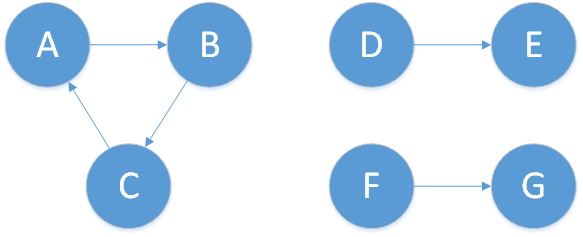
\includegraphics[width=0.4\textwidth]{Figure/Fig1.png}
		\caption{Relation graph}
		\label{fig:fig1}
	\end{figure}

From the figure we can conclude that the connect components are $(A,B,C)$, $(D,E)$ and $(F,G)$.
\subsection{R-13.2}
\noindent \emph{Question}: Let $G$ be a simple connected graph with $n$ vertices and $m$ edges. Explain why $O(\log m)$ is $O(\log n)$.

\noindent \emph{Answer}: When we have $m$ vertices, the maximum number of edges could be $m<n(n-1)<n^2$, which means $O(\log m)<O(\log n^2)= O(2\log n)=O(\log n)$. To sum up, $O(\log m)$ is $O(\log n)$.
\subsection{Given the graph}
\subsubsection{Draw the graph where all nodes are annotated with the order that they are visited in a \textbf{depth-first} search from A.}
\noindent \emph{Answer}: The result is shown in Fig. \ref{fig:fig2}.
	\begin{figure}[h]
		\centering
		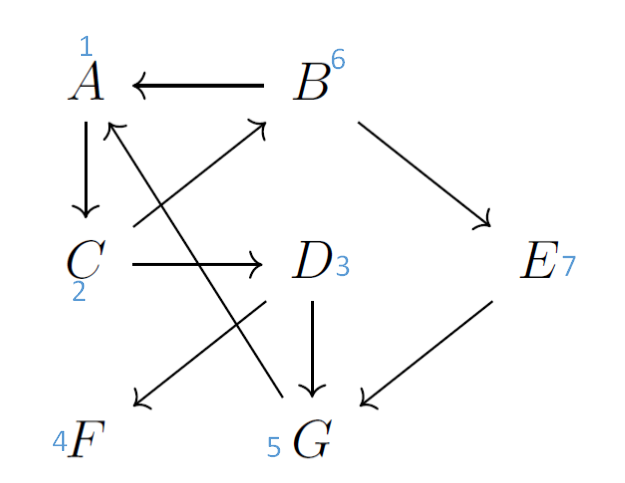
\includegraphics[width=0.4\textwidth]{Figure/Fig3.png}
		\caption{Annotated graph}
		\label{fig:fig2}
	\end{figure}
\subsubsection{Draw a representation of the tree generated by the DFS annotated over the previous part.}
\noindent \emph{Answer}: The result is shown in Fig. \ref{fig:fig3}.
	\begin{figure}[h]
		\centering
		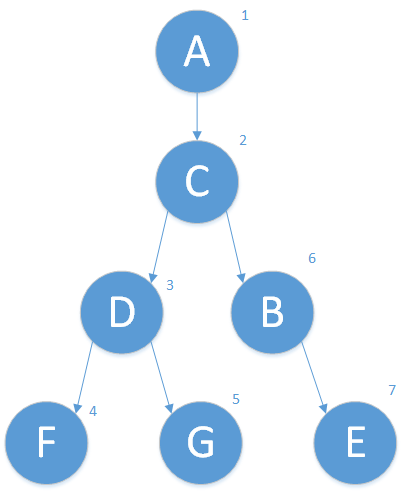
\includegraphics[width=0.4\textwidth]{Figure/Fig2.png}
		\caption{Tree graph}
		\label{fig:fig3}
	\end{figure}
\section{Application: Chess}
\noindent \emph{Answer}: To solve this problem in $O(n^2)$ time, we need to use the idea of Union-Find set to reduce the union time. 
\begin{algorithmic}
	\State \textbf{Algorithm} Chess($Table,n$)
	\State \textbf{Data}: The chess table $Table$, which is a two dimension table, and its one-dimensional size $n$.
	\State \textbf{Result}: A list of ordered pairs $(i,j)$ representing the positions of queens in the largest standoff.
	\State $Forest\gets$ empty union find forest
	\For{$i\gets 0$ to $n$}
		\For{$j\gets 0$ to $n$}
			\If {$Table[i][j]$}
				\State $Forest.Makeset(i,j)$ \Comment Make union-find set for every queen.
			\EndIf
		\EndFor
	\EndFor
	\For{$i\gets 0$ to $n$}
		\State $Temp \gets (-1,-1)$
		\For{$j\gets 0$ to $n$}
			\If{$Table[i][j]$}
				\If{$Temp \not = (-1,-1)$}
					\State $Union((i,j), Temp)$ \Comment Merge the queens in the same row 
				\EndIf
				\State $Temp \gets (i,j)$
			\EndIf
		\EndFor
	\EndFor
	\For{$i\gets 0$ to $n$}
		\State $Temp \gets (-1,-1)$
		\For{$j\gets 0$ to $n$}
			\If{$Table[j][i]$}
				\If{$Temp \not = (-1,-1)$}
					\State $Union((j,i), Temp)$ \Comment Merge the queens in the same column
				\EndIf
				\State $Temp \gets (j,i)$
			\EndIf
		\EndFor
	\EndFor
	\For{$i\gets 0$ to $2n-1$}
		\State $Temp \gets (-1,-1)$
		\For{$j\gets 0$ to $n-|n-i|$}
		\If{$i\leq n$}
			\State $x\gets n-i$
		\Else
			\State $x\gets 0$
		\EndIf
		\State $y \gets j$
			\If{$Table[x][y]$}
				\If{$Temp \not = (-1,-1)$}
					\State $Union((x,y), Temp)$ \Comment Merge the queens in the same diagonal
				\EndIf
				\State $Temp \gets (x,y)$
			\EndIf
		\EndFor
	\EndFor
	\For{$i\gets 0$ to $2n-1$}
		\State $Temp \gets (-1,-1)$
		\For{$j\gets 0$ to $n-|n-i|$}
			\If{$i\leq n$}
				\State $x\gets n-i$
			\Else
				\State $x\gets 0$
			\EndIf
				\State $y \gets j$
			\If{$Table[y][x]$}
				\If{$Temp \not = (-1,-1)$}
					\State $Union((y,x), Temp)$ \Comment Merge the queens in the same (other)diagonal
				\EndIf
				\State $Temp \gets (y,x)$
			\EndIf
		\EndFor
	\EndFor
	\State $MaxSize\gets 0$
	\State $MaxPos \gets 0$
	\For{$i\gets 0$ to $size(Forest)$}
		\If{$Forest[i].size()>MaxSize$}
			\State $MaxSize \gets Forest[i].size()$
			\State $MaxPos \gets i$
		\EndIf
	\EndFor
	
	\State \Return $Forest[MaxPos]$
\end{algorithmic}

	Since the union operation only cost $O(1)$ time, we can conclude that the `For' loops in the above pseudo-code all cost $O(n^2)$ time.
\section{Application: A World of Voxels}
\subsection{Describe a method to preprocess the array in $O(n\log(n))$ time.} 
\noindent \emph{Answer}: To preprocess the array and make such data structure in $O(n)$ size with the preprocess costing $O(n\log(b))$ time, we can use a tree structure, where a father node can have $6$ leaves, representing the up, down, front, behind, left and right block of a giving block. To create a tree, we can use both \textbf{DFS} and \textbf{BFS} to build the tree, they can both reveal the linked relationship but using \textbf{BFS} would better simulate the real metal block neighboring relationship, since in the real world, the longer the link is, the higher electrical resistance would be.
\begin{algorithmic}
	\State \textbf{Algorithm} BuildTree($Matrix,m,n,p$)
	\State \textbf{Data}: A matrix representing the metal blocks, and its three dimensional size $m,n,p$
	\State \textbf{Result}: The tree represent of the metal blocks.
	\State $Root\gets (-1,-1,-1)$
	\State $Roots\gets$ empty list \Comment the list of roots
	\For{$i \gets 0$ to $m$}
		\For{$j \gets 0$ to $n$}
			\For{$k \gets 0$ to $p$}
				\State $Visited[i][j][k] \gets Matrix[i][j][k]$ \Comment Copy to make a `visited' matrix.
				\If{$Matrix[i][j][k]$}
					\State $Root \gets (i,j,k)$ \Comment Find the root node
					\State $Roots.append(Root)$
					\State $Root.father \gets NULL$
					\State $RecursiveBuildTree(Martix,Visit,Root[0],Root[1],Root[2],m,n,p)$
				\EndIf
			\EndFor
		\EndFor
	\EndFor

\\
	\State \textbf{def} $RecursiveBuildTree(Matrix,Visit,i,j,k,m,n,p)$
	\State $Root \gets(i,j,k)$
	\If{$i+1<m$} 
		\If{$Matrix[i+1][j][k]$ and $Visit[i+1][j][k]$} \Comment first dimension plus one
			\State $Root.link[0] \gets (i+1,j,k)$
			\State $Visit[i+1][j][k]\gets 0$
			\State $Node[i+1][j][k].father \gets Root$
		\EndIf
	\EndIf
	\If{$j+1<n$} 
		\If{$Matrix[i][j+1][k]$ and $Visit[i][j+1][k]$} \Comment second dimension plus one
			\State $Root.link[1] \gets (i,j+1,k)$
			\State $Visit[i][j+1][k]\gets 0$
			\State $Node[i][j+1][k].father \gets Root$
		\EndIf
	\EndIf
	\If{$k+1<p$} 
		\If{$Matrix[i][j][k+1]$ and $Visit[i][j][k+1]$} \Comment third dimension plus one
			\State $Root.link[2] \gets (i,j,k+1)$
			\State $Visit[i][j][k+1]\gets 0$
			\State $Node[i][j][k+1].father \gets Root$
		\EndIf
	\EndIf
	\If{$i-1\geq 0$} 
		\If{$Matrix[i-1][j][k]$ and $Visit[i-1][j][k]$} \Comment first dimension minus one
			\State $Root.link[3] \gets (i-1,j,k)$
			\State $Visit[i-1][j][k]\gets 0$
			\State $Node[i-1][j][k].father \gets Root$
		\EndIf
	\EndIf
	\If{$j-1\geq 0$} 
		\If{$Matrix[i][j-1][k]$ and $Visit[i][j-1][k]$} \Comment second dimension minus one
			\State $Root.link[4] \gets (i,j-1,k)$
			\State $Visit[i][j-1][k]\gets 0$
			\State $Node[i][j-1][k].father \gets Root$
		\EndIf
	\EndIf
	\If{$k-1\geq 0$} 
		\If{$Matrix[i][j][k-1]$ and $Visit[i][j][k-1]$} \Comment third dimension minus one
			\State $Root.link[5] \gets (i,j,k-1)$
			\State $Visit[i][j][k-1]\gets 0$
			\State $Node[i][j][k-1].father \gets Root$
		\EndIf
	\EndIf
	\For{$i\gets 0$ to $5$}
		\If{$Root.link[i]\not = NULL$}
			\State $RecursiveBuildTree(Matrix,Visit,Root.link[i][0],Root.link[i][1],Root.link[i][2],m,n,p)$
		\EndIf
	\EndFor
\end{algorithmic}

Since in this algorithm, we are using a tree to represent the linking relationship. $Node[i][j][k]$ here represents the node with position $(i,j,k)$. To find whether two given block is connected, we can run the algorithm which can find the root node:
\begin{algorithmic}
	\State \textbf{Algorithm} IsConnected($i_1,j_1,k_1,i_2,j_2,k_2$)
	\State \textbf{Data}: The position of two blocks $(i_1,j_1,k_1)$ and $(i_2,j_2,k_2)$
	\State \textbf{Result}: Whether the two blocks are connected.
	\State \Return $FindRoot(i_1,j_1,k_1)=FindRoot(i_2,j_2,k_2)$\Comment Return whether the root of this two blocks are same
\\
	\State \textbf{def} $FindRoot(i,j,k)$
	\If{$Node[i][j][k].father \not = NULL$}
		\State \Return $FindRoot(i,j,k)$
	\Else
		\State \Return $(i,j,k)$
	\EndIf
\end{algorithmic}

Since the depth of the tree is at most $O(\log n)$, this query function can at most reach the $O(\log n)$ time complexity.
\subsection{Describe how to support additions, what is the asymptotic runtime of an addition?}
\noindent \emph{Answer}: To add a new block in this tree, we need first to find whether there is any block in other tree that is a neighbor of this tree and, may be merge two trees into one. The algorithm is shown as follow:
\begin{algorithmic}
	\State \textbf{Algorithm} AddBlock($i,j,k,m,n,p$)
	\State $LinkedTree\gets$ empty list
	\If{$i+1<m$} 
		\If{$FindRoot(i+1,j,k)\not = (i,j,k)$} \Comment Is in a tree
			\State $LinkedTree.append(i,j,k)$
			\State $Node[i+1,j,k].linked[3] \gets (i,j,k)$
			\State $Node[i,j,k].father \gets (i+1,j,k)$
		\EndIf
	\EndIf
	\If{$j+1<n$} 
		\If{$FindRoot(i,j+1,k)\not = (i,j,k)$} \Comment Is in a tree
			\State $LinkedTree.append(i,j,k)$
			\State $Node[i,j,k].linked[4] \gets (i,j,k)$
			\State $Node[i,j,k].father \gets (i,j+1,k)$
		\EndIf
	\EndIf
	\If{$k+1<p$} 
		\If{$FindRoot(i,j,k+1)\not = (i,j,k)$} \Comment Is in a tree
			\State $LinkedTree.append(i,j,k)$
			\State $Node[i,j,k+1].linked[5] \gets (i,j,k)$
			\State $Node[i,j,k].father \gets (i,j,k+1)$
		\EndIf
	\EndIf
	\If{$i-1\geq 0$} 
		\If{$FindRoot(i-1,j,k)\not = (i,j,k)$} \Comment Is in a tree
			\State $LinkedTree.append(i,j,k)$
			\State $Node[i-1,j,k].linked[0] \gets (i,j,k)$
			\State $Node[i,j,k].father \gets (i-1,j,k)$
		\EndIf
	\EndIf
	\If{$j-1\geq 0$} 
		\If{$FindRoot(i,j-1,k)\not = (i,j,k)$} \Comment Is in a tree
			\State $LinkedTree.append(i,j,k)$
			\State $Node[i,j-1,k].linked[1] \gets (i,j,k)$
			\State $Node[i,j,k].father \gets (i,j-1,k)$
		\EndIf
	\EndIf
	\If{$k-1\geq 0$} 
		\If{$FindRoot(i,j,k-1)\not = (i,j,k)$} \Comment Is in a tree
			\State $LinkedTree.append(i,j,k)$
			\State $Node[i,j,k-1].linked[2] \gets (i,j,k)$
			\State $Node[i,j,k].father \gets (i,j,k-1)$
		\EndIf
	\EndIf
	\If{$LinkedTree.size()>1$}
		\For{$i\gets1$ to $LinketTree.size()$}
			\State $Node[i,j,k].linked[5+i] = LinkedTree[i]$
			\State $LinkedTree[i].father \gets (i,j,k)$ \Comment NOTE: This might destroy the original relationship of neighboring, but will keep the union-find feature.
		\EndFor
	\EndIf
\end{algorithmic}

As is shown in the algorithm above, the time of an addition should be $O(1)$. But if we want to keep the neighboring relationship in the tree, we may need to transverse the tree and cost more time. However, it is not required in this question to keep such relationship so the time costing can be reduced.
\subsection{Describe a way to support deletions of blocks, also describe any practical problems with the runtime of your method.}
\noindent \emph{Answer}: To remove a block, we can simply remove the block from the tree and make other adjacent blocks be the root of a new tree if the new tree will never be connected to the original tree. However, as the tree we described above may not represent all the neighboring relationship, we will have to infer such relationship using the index of all the remaining blocks in the forest. Such approach will achieve a time costing of $O(n^2)$ because it may need to compare every pair of blocks to verify if they are adjacent. Such time costing is much larger than the building tree approach as described in question 8.1. Thus my approach of removing a block would be remove the block out of the original matrix $Matrix$ and then rebuild the tree.
\section{Graph on a Grid}
\subsection{Show the adjacency list representation of the following graph.}
\noindent \emph{Answer}: The adjacency list is shown as follow:

$(2,2) \to (1,2), (2,1), NULL$

$(2,1) \to (1,1), (2,0), NULL$

$(1,2) \to (1,1), (0,2), NULL$

$(1,1) \to (1,0), (0,1), NULL$

$(2,0) \to (1,0), NULL$

$(0,2) \to (0,1), NULL$

$(0,1) \to (0,0), NULL$

$(1,0) \to (0,0), NULL$

$(0,0) \to NULL$

\subsection{Show two different depth-first traversals from $(2,2)$ on the graph in part a.}
\noindent \emph{Answer}: First DFS:$(2,2),(1,2),(0,2),(0,1),(0,0),(1,1),(1,0),(2,1),(2,0)$.\\Second DFS:$(2,2),(2,1),(2,0),(1,0),(0,0),(1,1),(0,1),(1,2),(0,2)$.
\section{EECS 454 only}
\subsection{C-17.4}
\noindent \emph{Question}: Show that every language $L$ in \textbf{P} is polynomial-time reducible to the language $M = {5}$, that is, the language that simply asks whether the binary encoding of
the input is equal to $5$.
\subsection{C-17.5}
\noindent \emph{Question}: Show how to construct a Boolean circuit $C$ such that, if we create variables only for the inputs of $C$ and then try to build a Boolean formula that is equivalent to
C, then we will create a formula exponentially larger than an encoding of $C$.

\noindent \emph{Hint}: Use recursion to repeat subexpressions in a way that doubles their size each time they are used.
\end{document}